\section{Ceph Block Device}

%\begin{frame}{Ceph Block Device - RBD}
%    \begin{itemize}
%        \item Block devices are the most common way to store data
%        \item Allows for storage of virtual disks in the Ceph Object Store
%        \item Allows decoupling of VMs and containers
%        \item High-Performance through data striping across the cluster
%        \item Boot support in QEMU, KVM, and OpenStack(Cinder)
%        \item Mount support in the Linux Kernel
%    \end{itemize}
%\end{frame}

\begin{frame}[fragile]{Create and Mount RBD}
\begin{lstlisting}[language=python]
# create a block device pool
$ ceph osd pool create rbd 128 
$ rbd pool init

# create a block device image(1024MB)
$ rbd create --size 1024 foo
$ rbd list
foo

# map a block device
$ sudo rbd device map rbd/foo --id admin
/dev/rbd0
$ rbd device list
id pool image snap device
0  rbd  foo   -    /dev/rbd0

# format the block device and create a file system
$ sudo mkfs.ext4 -m0 /dev/rbd0
$ sudo mkdir /mnt/rbd
$ sudo mount /dev/rbd/rbd/foo /mnt/rbd

# 查看挂载情况
$ df -h
...
/dev/rbd0            976M  2.6M  958M    1% /mnt/rbd
\end{lstlisting}
\end{frame}

\begin{frame}{RBD: Native}
    \begin{figure}[htpb]
        \centering
        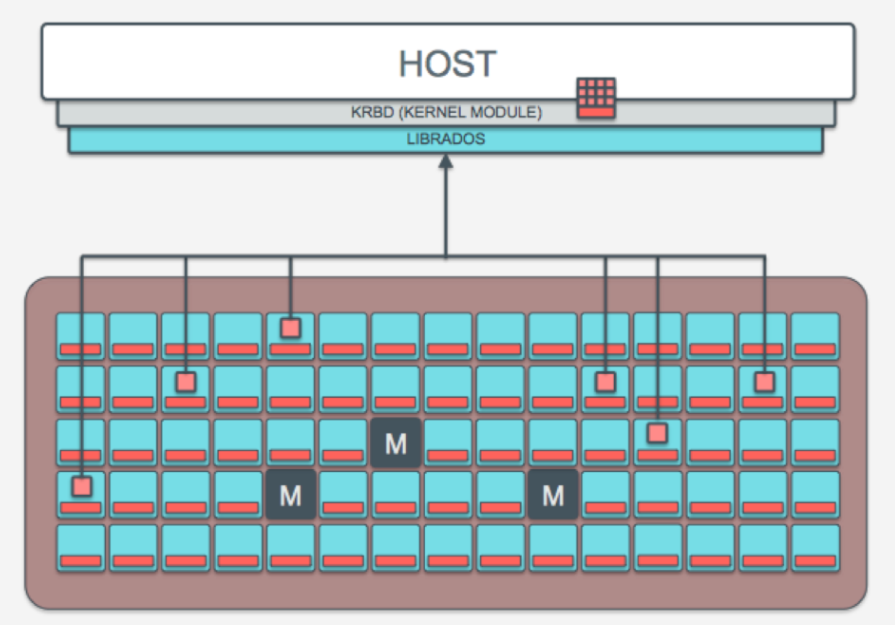
\includegraphics[width=0.7\linewidth]{rbd-native.png}
    \end{figure}
    \textbf{Machines can mount an RBD image using native linux kernel drivers} 
\end{frame}

\begin{frame}{RBD: Virtual Machines}
    \begin{itemize}
        \item \textbf{The \textit{librbd} library}
            \begin{itemize}
                \item Maps data blocks into objects for storage in the Ceph Object Store
                \item Inherit \textit{librados} capabilities such as snapshots and clones
            \end{itemize}
        \item \textbf{Virtualization containers}
            \begin{itemize}
                \item KVM or QEMU can use VM images that are stored in RADOS
                \item Virtualization containers can also use RBD block storage in OpenStack and CloudStack platforms
            \end{itemize}
        \item \textbf{Ceph based VM Images}
            \begin{itemize}
                \item Are striped across the entire cluster
                \item Allow simultaneous read access from different cluster nodes
            \end{itemize}
    \end{itemize}
\end{frame}

\begin{frame}{RBD: Virtual Machines}
    \begin{figure}[htpb]
        \centering
        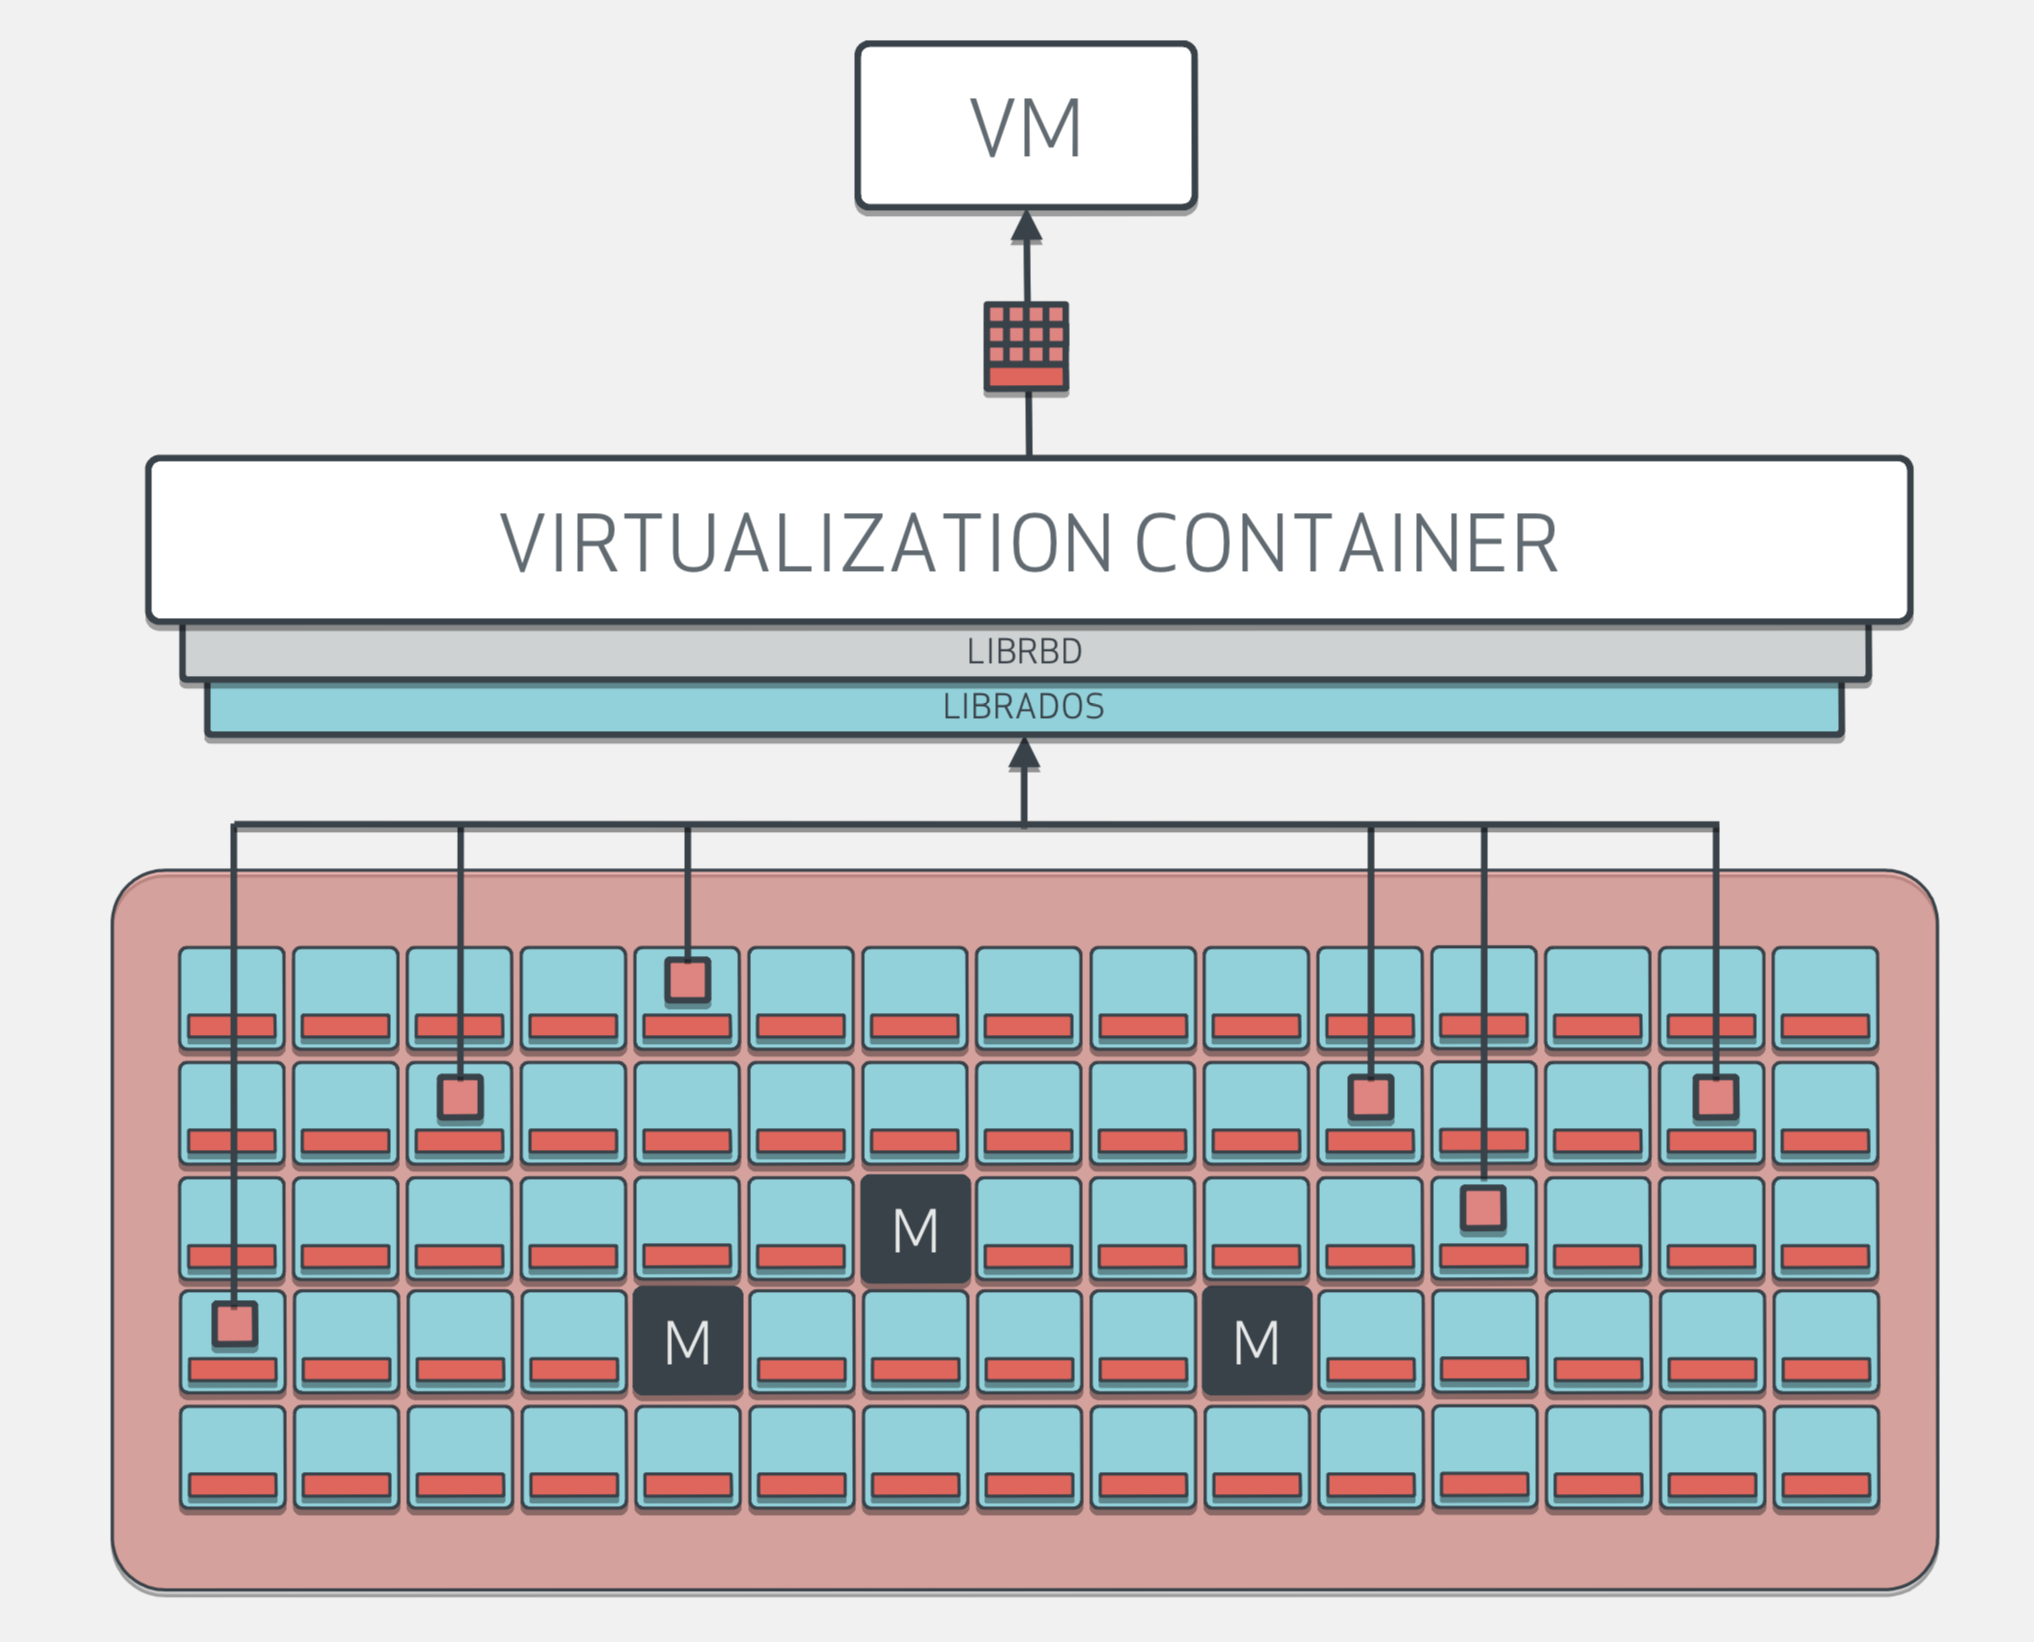
\includegraphics[width=0.7\linewidth]{rbd-vm.png}
    \end{figure}
\end{frame}

\begin{frame}[fragile]{Access RBD using librbd}
\begin{lstlisting}[language=python]
with rados.Rados(conffile='my_ceph.conf') as cluster:
    with cluster.open_ioctx('mypool') as ioctx:
        rbd_inst = rbd.RBD()
        size = 4 * 1024**3  # 4 GiB
        rbd_inst.create(ioctx, 'myimage', size)
        with rbd.Image(ioctx, 'myimage') as image:
            data = 'foo' * 200
            image.write(data, 0)
\end{lstlisting}
\end{frame}

\begin{frame}[fragile]
\begin{columns}
    \begin{column}{0.4\textwidth}
\begin{lstlisting}[language=python]
apiVersion: v1
kind: PersistentVolume
metadata:
  name: ceph-rbd-pv
spec:
  capacity:
    storage: 1Gi
  accessModes:
    - ReadWriteOnce
  rbd:
    monitors:
    - '172.31.56.105:6789'
    - '172.31.57.232:6789'
    - '172.31.58.195:6789'
    pool: rbd
    image: foo
    user: admin
    secretRef:
      name: ceph-secret
    fsType: ext4
    readOnly: false
\end{lstlisting}
    \end{column}
    \begin{column}{0.4\textwidth}
\begin{lstlisting}[language=python]
apiVersion: v1
kind: PersistentVolumeClaim
metadata:
  name: ceph-rbd-pv-claim
spec:
  accessModes:
    - ReadWriteOnce
  resources:
    requests:
      storage: 1Gi
\end{lstlisting}

\begin{lstlisting}[language=python]
apiVersion: v1
kind: Pod
metadata:
  name: ceph-rbd-pv-pod1
spec:
  containers:
  - name: rbd-rw
    image: kubernetes/pause
    volumeMounts:
    - name: ceph-rbd-vol1
      mountPath: /mnt/rbd
      readOnly: false
  volumes:
  - name: ceph-rbd-vol1
    persistentVolumeClaim:
      claimName: ceph-rbd-pv-claim
\end{lstlisting}
    \end{column}
\end{columns}
\end{frame}

